\documentclass[letterpaper]{article}
\usepackage[submission]{aaai2027}
\usepackage[hyphens]{url}
\usepackage{graphicx}
\urlstyle{rm}
\def\UrlFont{\rm}
\usepackage{natbib}
\usepackage{caption}
\frenchspacing
\usepackage{amsmath}
\usepackage{amssymb}
\usepackage{booktabs}
\usepackage{xcolor}
\usepackage{pgfplots}
\usetikzlibrary{arrows.meta}
\pgfplotsset{
    compat=1.18,
    expplot/.style={
        width=\columnwidth,
        tick label style={font=\footnotesize},
        xlabel style={font=\footnotesize},
        ylabel style={font=\footnotesize},
        legend style={font=\footnotesize, draw=none},
        every axis plot/.append style={thick, mark size=2.5pt},
        tick style={black},
        axis line style={black},
    },
}

% Tableau 10 colors
\definecolor{tab-blue}{HTML}{4E79A7}
\definecolor{tab-orange}{HTML}{F28E2B}
\definecolor{tab-red}{HTML}{E15759}
\definecolor{tab-teal}{HTML}{76B7B2}
\definecolor{tab-green}{HTML}{59A14F}
\definecolor{tab-gray}{HTML}{BAB0AC}
\definecolor{lr-blue}{HTML}{78A6D6}
\definecolor{lr-red}{HTML}{F08080}

\newcommand{\acc}{\textsc{Acc}}
\newcommand{\con}{\textsc{Con}}
\newcommand{\ccal}{\textsc{Cal}}
\newcommand{\multirow}[3]{#3}
\pdfinfo{
/TemplateVersion (2027.1)
}
\setcounter{secnumdepth}{0}

\title{Position Shortcuts in Reinforcement-Trained LLM Judges}

\author{Anonymous Submission}
\affiliations{}

\begin{document}
\tolerance=1500
\emergencystretch=3em
\hbadness=3000
\maketitle

\begin{abstract}
LLM judges are increasingly trained to evaluate pairwise preferences and to provide reward signals in post-training pipelines. We show that standard accuracy can overstate judge quality when preference data are converted into fixed-order judge prompts: if a \texttt{chosen} response is always rendered as Response A, response position becomes a perfect predictor of the gold verdict. Trained judges can then improve original-order accuracy by learning a position shortcut rather than comparing the responses. We diagnose this failure with position-swap evaluation across SFT, DPO, GRPO, reward variants, label schemes, learning rates, and model families. On unbalanced data, training improves original-order accuracy while degrading swap accuracy and position-swap consistency; in the most extreme case, a judge reaches 99\% original-order accuracy by almost always selecting the first response. Balancing preferred responses across positions removes the position-label correlation, restores consistency, and retains non-positional accuracy gains in our evaluated settings. These results motivate reporting position-swap consistency alongside accuracy for reinforcement-trained LLM judges.
\end{abstract}

% ===========================================================================
\section{Introduction}
% ===========================================================================

LLM judges are increasingly trained to evaluate pairwise preferences and to provide reward signals in post-training pipelines~\citep{zheng2023judging,zheng2024arena}. These judges are usually optimized and reported by accuracy: whether their verdict matches a gold preference label. This metric carries an implicit assumption: the model should match the label for the same reason the label was assigned, namely evidence that one response better satisfies the prompt. If prompt construction introduces artifacts that also predict the label, standard optimization can amplify those artifacts instead. This creates a basic question for trained judges: when accuracy improves, has the model learned to compare the responses, or has it learned a shortcut in the training interface?

We identify one such shortcut created by standard preference-data preprocessing. Preference datasets often store examples as \texttt{chosen}/\texttt{rejected}. When a conversion script renders \texttt{chosen} as Response A and \texttt{rejected} as Response B, the preferred response becomes Response A for every training instance. Position therefore becomes a perfect predictor of the training label under that prompt construction. Any objective that rewards label matching can exploit this regularity by learning a positional policy rather than comparing the responses: apparent accuracy rises, while position-swap consistency collapses. Figure~\ref{fig:mechanism} gives the intuition.

\begin{figure*}[t]
\centering
\includegraphics[width=0.96\textwidth]{figure1.pdf}
\caption{The position shortcut and the data-level fix. When the preferred response is always rendered first, RL can obtain high reward by learning a positional rule rather than comparing response quality. Balancing response order removes the global position-label correlation and makes a first-position rule uninformative.}
\label{fig:mechanism}
\end{figure*}

We diagnose this failure with position-swap evaluation: for each pair, the judge must give logically equivalent verdicts before and after the two responses are swapped. This separates apparent accuracy from position-invariant judgment. Across SFT, DPO, and GRPO; accuracy-only, decisiveness, calibration, and composite rewards; and prompt, label, learning-rate, and model-family controls, we find the same accuracy-consistency dissociation: optimization makes judges look better under the original ordering while making them less stable under position swap. In the strongest failure mode, high original-order accuracy is explained almost entirely by first-position selection rather than content comparison. The controls change the severity but do not remove the shortcut in our experiments, pointing to the training data layout as the structural source.

This points to a data-level intervention: balance the training data so that preferred responses appear equally often in both positions. Balanced training removes the position-reward correlation, restores consistency to the untrained baseline range, and retains modest genuine gains for GRPO while giving stronger gains under balanced SFT. Comparing unbalanced and balanced training provides an operational decomposition of apparent improvement into content-based gain and shortcut gain, estimating that position exploitation accounts for 11.0 percentage points in the primary Qwen2.5-7B setting and 17.4 percentage points for Mistral-7B.

Our contributions:
\begin{itemize}
\item We identify a training-interface shortcut in pairwise LLM judge training: naive \texttt{chosen}/\texttt{rejected}-to-A/B preprocessing can make response position a perfect predictor of the gold verdict, allowing trained judges to improve apparent accuracy without learning the intended comparison.
\item We introduce position-swap evaluation as a diagnostic for separating apparent accuracy from position-invariant judgment, and show a repeated accuracy-consistency dissociation across training algorithms, reward designs, prompt and label controls, learning rates, and model families.
\item We evaluate balanced response positions as a data-level intervention that cancels the first-order shortcut gradient, restores position-swap consistency, and enables a decomposition of apparent accuracy into genuine judgment gain and positional shortcut gain.
\end{itemize}

% ===========================================================================
\section{Related Work}
% ===========================================================================

\paragraph{Bias and Consistency in LLM Judges.}
Prior work has shown that LLM judges are sensitive to where candidate responses appear in a pairwise prompt~\citep{zheng2023judging,wang2024largelanguagemodels,zhu2024judgebench}. This position bias interacts with broader evaluator biases, including length preference, self-preference, and reliance on surface features~\citep{wu2024style,koo2024benchmarking,li2024quantifying,park2024disentangling,singhal2024long}. Existing work therefore develops metrics and protocols for measuring or mitigating inconsistent judgments, such as swap-based consistency analysis, BT-$\sigma$~\citep{btsigma2026}, inference-time consistency checks~\citep{trustjudge2026}, permutation-aware RL objectives~\citep{eisgrpo2026,pagrpo2026}, and selective abstention for uncertain pairwise judgments~\citep{scope2026}. These studies establish that position sensitivity matters. Our focus is the training-time source: standard preference-data conversion can make response position a rewarded feature before any evaluation-time correction is applied.

\paragraph{RL Training for Preference Judges.}
Preference learning has long used human judgments to train language models~\citep{christiano2017deep,stiennon2020learning,ouyang2022training,bai2022training}, and recent work applies similar optimization recipes to the judges themselves. JudgeLRM~\citep{chen2025judgelrm} trains reasoning judges with GRPO~\citep{shao2024deepseekmath}; FairJudge~\citep{fairjudge2026} combines SFT, DPO~\citep{rafailov2023direct}, and GRPO with consistency-oriented objectives. These approaches treat reward design or algorithmic consistency constraints as the main levers for improving judge behavior. We instead ask whether the data layout makes a non-semantic feature predictive of reward. Under a position confound, even a correct label reward can be maximized by selecting the first response, so reported accuracy gains must be checked against position-swap consistency.

\paragraph{Shortcut Learning in Neural Networks.}
Shortcut learning is a well-documented failure mode in which models exploit spurious data correlations rather than acquiring task-relevant features~\citep{geirhos2020shortcut,mccoy2019right,tu2020empirical}. When a confound perfectly predicts the label, models may learn the confound. Standard mitigations include data augmentation, adversarial training, and causal intervention. In the RLHF setting, reward hacking~\citep{skalse2022defining,gao2023scaling,pan2024spontaneous} describes a related failure where models exploit flaws in the reward model, and constrained RL~\citep{moskovitz2024confronting} proposes multi-objective solutions. Our setting highlights a complementary case: the label-matching reward can be correct with respect to the annotation, yet still reinforce a non-semantic route to that label. We show that the tested proxy rewards do not resolve the data-level position confound, while balancing response positions removes the simplest positional reward path.

% ===========================================================================
\section{Diagnostic Framework}
% ===========================================================================

\subsection{Pairwise Judge Training and the Position Confound}

We study LLM judges trained to evaluate pairwise preferences. Given a query $q$ and two candidate responses, the judge produces a rationale, a verdict $v \in \{A, B, \text{tie}\}$, and a confidence score $c \in [0, 1]$. The intended behavior is comparative judgment: the verdict should follow evidence about which response better satisfies the prompt, not incidental artifacts of the prompt interface.

The artifact we study is response position. The position confound arises when preference data are converted into pairwise judge prompts. In standard \texttt{chosen}/\texttt{rejected} datasets, the preferred response is stored in the \texttt{chosen} field. In our RewardBench-to-judge-prompt conversion~\citep{lambert2024rewardbench}, \texttt{chosen} is rendered as Response A and \texttt{rejected} as Response B, so the gold label is ``A'' for every training instance. Position is therefore perfectly correlated with reward: under an accuracy reward, selecting Response A always receives maximum reward.

This makes apparent accuracy ambiguous. A trained judge can improve by learning comparison-relevant evidence, by learning the positional feature, or by mixing both. Evaluation on the same ordering cannot separate these sources, because the shortcut and the intended task produce the same label. The position confound is therefore not an artificial perturbation introduced only at evaluation time; it is inherited from the prompt-construction rule used to build the judge-training data.

\subsection{Training Conditions}

We compare two training conditions. In the \emph{unbalanced} condition, the prompt conversion renders \texttt{chosen} as Response A for every training pair, so the gold verdict is always ``A.'' We then vary the optimization recipe while keeping this confound fixed: SFT, DPO, GRPO with an accuracy reward, and GRPO with decisiveness, calibration, and composite reward variants. These variants are stress tests for whether common proxy rewards are sufficient to induce comparative judgment under a fixed position-label correlation.

In the \emph{balanced} condition, preferred responses appear in position A for half of the training instances and position B for the other half. Unless otherwise stated, we create this condition by adding a swapped mirror of each training pair and flipping the gold label. We verify in the supplementary material that the effect is not due to dataset duplication. Once position A is correct exactly half the time, a global first-position rule cannot explain gains over the untrained model.

We use Qwen2.5-7B-Instruct~\citep{qwen2025qwen25} as the primary model and replicate key conditions on Qwen3-8B~\citep{qwen2025qwen3} and Mistral-7B-Instruct-v0.3~\citep{jiang2023mistral}. GRPO uses LoRA~\citep{hu2022lora} over attention projections for 500 steps; full data construction, reward definitions, hyperparameters, and seeds are in the supplementary material.

\subsection{Position-Swap Evaluation}

We evaluate each model on 449 held-out test instances, generating responses with temperature 0.1 and max 512 new tokens. For each instance, we generate judgments on both the original and position-swapped order. This creates a direct test of whether the judge's verdict follows the compared responses or their positions.

We report five metrics:
\begin{itemize}
\item \textbf{Original-order accuracy}: agreement with gold labels on the original ordering.
\item \textbf{Swap accuracy}: agreement with the flipped gold label after the two responses are swapped.
\item \textbf{Position consistency}: the fraction of instances where the verdict is logically equivalent under position swap. If the model predicts A on the original order, it should predict B on the swapped order, and vice versa. Ties are self-consistent.
\item \textbf{First-position rate}: the fraction of original and swapped judgments that select the first-listed response.
\item \textbf{Position bias}: the percentage-point gap between always-first and always-second inconsistent predictions.
\end{itemize}

Position consistency and swap accuracy are the critical diagnostics because they distinguish position-invariant judgment from position-dependent shortcut use. Original-order accuracy alone is reported only as apparent accuracy under the confounded order. We treat ties as self-consistent because a tie verdict is unchanged by swapping response order. Paired tie-only cases are not the driver of the effect: under a stricter tie-as-inconsistent check, the key trained-model consistency comparisons move by at most about one point and conclusions are unchanged. For multi-seed conditions, tables report mean $\pm$ standard deviation across seeds.

% ===========================================================================
\section{Experiments}
% ===========================================================================

\subsection{Unbalanced Training Creates an Accuracy-Consistency Split}

We first ask whether RL training exploits the prompt artifact created by the standard conversion from preference data to judge prompts, where every training label is ``A.''

\begin{table}[t]
\centering
\scriptsize
\setlength{\tabcolsep}{2.0pt}
\resizebox{\columnwidth}{!}{%
\begin{tabular}{lccccc}
\toprule
\textbf{Method} & \textbf{Orig Acc} $\uparrow$ & \textbf{Swap Acc} $\uparrow$ & \textbf{Con} $\uparrow$ & \textbf{First-pos} & \textbf{Bias} $\downarrow$ \\
\midrule
Baseline (no training) & 80.2 & 75.3 & 81.5 & 49.3 & 2.4 \\
\midrule
SFT & 100.0 & 0.0 & 0.0 & 100.0 & 100.0 \\
DPO & 94.2 & 50.3 & 54.3 & 69.4 & 40.8 \\
GRPO Acc-only & 94.7{\scriptsize$\pm$0.7} & 55.7{\scriptsize$\pm$6.4} & 59.8{\scriptsize$\pm$7.6} & 68.1{\scriptsize$\pm$3.6} & 37.5{\scriptsize$\pm$7.9} \\
\quad + Decisive & 93.9{\scriptsize$\pm$1.1} & 61.0{\scriptsize$\pm$5.4} & 66.3{\scriptsize$\pm$6.5} & 65.0{\scriptsize$\pm$3.5} & 31.3{\scriptsize$\pm$6.8} \\
\quad + Calibration & 95.4{\scriptsize$\pm$0.5} & 53.1{\scriptsize$\pm$7.4} & 56.1{\scriptsize$\pm$7.9} & 69.4{\scriptsize$\pm$4.0} & 40.3{\scriptsize$\pm$7.9} \\
\quad + Both (Full) & 94.7{\scriptsize$\pm$0.9} & 54.8{\scriptsize$\pm$8.3} & 58.7{\scriptsize$\pm$9.1} & 68.8{\scriptsize$\pm$4.3} & 38.6{\scriptsize$\pm$9.1} \\
\midrule
GRPO Full (lr=1e-5) & 98.9 & 37.0 & 38.1 & 80.5 & 61.5 \\
GRPO Full (lr=1e-6) & 83.7 & 76.2 & 83.3 & 51.0 & 5.6 \\
\bottomrule
\end{tabular}
}
\caption{Unbalanced training (gold = ``A''). All methods increase original-order accuracy while losing swap accuracy, position-swap consistency, and position neutrality. Position bias is the percentage-point gap between always-first and always-second inconsistent predictions.}
\label{tab:unbalanced}
\end{table}

Table~\ref{tab:unbalanced} shows the central dissociation. Training improves original-order accuracy, but the gain is accompanied by lower swap accuracy, a large loss in position-swap consistency, and a sharp increase in first-position selection. The methods differ in how completely the shortcut takes over: SFT reaches the degenerate endpoint of perfect original-order accuracy with zero swap accuracy and zero consistency, while DPO and GRPO retain more comparison signal but still move toward stronger position dependence.

Reward variants and learning rate changes modulate this tradeoff without removing it in our experiments. The best tested reward-only mitigation improves consistency only partially and remains below the untrained baseline. Similarly, conservative learning rates can mask the shortcut by limiting optimization pressure, but once the learning rate crosses a threshold documented in the supplementary material, original-order accuracy increases by trading off swap accuracy and position-swap consistency. These interventions change when and how strongly the shortcut appears; they do not remove the underlying confound.

These results point back to the data: under the tested training methods, proxy rewards, and learning rates, the most reliable mitigation is to remove the position-label correlation before optimization.

\subsection{Balanced Data Restores Position-Invariant Judgment}

We therefore train with balanced data where preferred responses appear equally in both positions (Table~\ref{tab:balanced}).

\begin{table}[t]
\centering
\scriptsize
\setlength{\tabcolsep}{2.0pt}
\resizebox{\columnwidth}{!}{%
\begin{tabular}{lccccc}
\toprule
\textbf{Method} & \textbf{Orig Acc} $\uparrow$ & \textbf{Swap Acc} $\uparrow$ & \textbf{Con} $\uparrow$ & \textbf{First-pos} & \textbf{Bias} $\downarrow$ \\
\midrule
Baseline (no training) & 80.2 & 75.3 & 81.5 & 49.3 & 2.4 \\
\midrule
SFT Balanced & 91.3 & 89.1 & 87.1 & 51.1 & 2.2 \\
GRPO Acc-only Bal. & 84.0{\scriptsize$\pm$1.8} & 80.8{\scriptsize$\pm$1.4} & 84.4{\scriptsize$\pm$0.4} & 50.3{\scriptsize$\pm$0.5} & 2.3{\scriptsize$\pm$1.2} \\
GRPO Decisive Bal. & 82.9{\scriptsize$\pm$0.6} & 79.9{\scriptsize$\pm$1.5} & 83.4{\scriptsize$\pm$1.4} & 50.1{\scriptsize$\pm$0.5} & 2.4{\scriptsize$\pm$1.5} \\
GRPO Calibration Bal. & 83.4{\scriptsize$\pm$1.1} & 79.5{\scriptsize$\pm$1.0} & 83.0{\scriptsize$\pm$1.3} & 50.5{\scriptsize$\pm$0.5} & 3.0{\scriptsize$\pm$0.8} \\
GRPO Full Balanced & 83.7{\scriptsize$\pm$1.1} & 81.4{\scriptsize$\pm$1.6} & 84.0{\scriptsize$\pm$0.8} & 50.0{\scriptsize$\pm$1.0} & 1.5{\scriptsize$\pm$2.2} \\
\bottomrule
\end{tabular}
}
\caption{Balanced training (gold = 50\% A, 50\% B). Data deconfounding keeps first-position selection near 50\%, restores consistency, and makes original-order and swap accuracy much closer.}
\label{tab:balanced}
\end{table}

\begin{figure}[t]
\centering
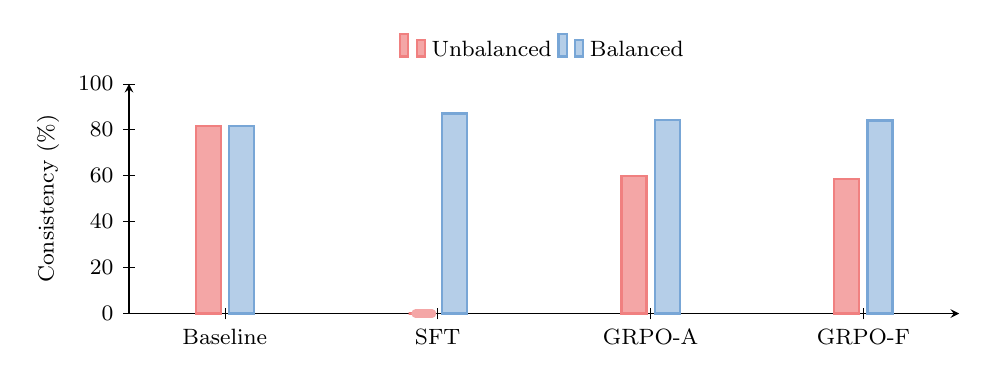
\begin{tikzpicture}
\begin{axis}[
    expplot,
    height=4.5cm,
    ybar=3pt,
    bar width=9pt,
    ylabel={Consistency (\%)},
    symbolic x coords={Baseline, SFT, Acc, Full},
    xtick=data,
    xticklabels={Baseline, SFT, GRPO-A, GRPO-F},
    ymin=0, ymax=100,
    ytick={0,20,40,60,80,100},
    grid=none,
    legend style={at={(0.5,1.05)}, anchor=south, legend columns=2},
    axis lines=left,
    enlarge x limits=0.15,
    clip=false,
]
\addplot[fill=lr-red!70, draw=lr-red] coordinates {(Baseline,81.5) (SFT,0.0) (Acc,59.8) (Full,58.7)};
\addlegendentry{Unbalanced}
\addplot[fill=lr-blue!55, draw=lr-blue] coordinates {(Baseline,81.5) (SFT,87.1) (Acc,84.4) (Full,84.0)};
\addlegendentry{Balanced}
\draw[lr-red!70, line width=3pt, line cap=round] ([xshift=-8pt]axis cs:SFT,0) -- ([xshift=-2pt]axis cs:SFT,0);
\end{axis}
\end{tikzpicture}
\caption{Balanced data restores consistency. Red bars show unbalanced training; light-blue bars show balanced training, with the baseline repeated for reference. The SFT red tick marks 0\% consistency. GRPO-A and GRPO-F denote accuracy-only and full-composite GRPO.}
\label{fig:fix}
\end{figure}

Balanced training reverses the pattern. Models trained on balanced data keep consistency and position bias near the untrained baseline, rather than trading consistency for apparent original-order accuracy (Figure~\ref{fig:fix}). The original-order accuracy gap between unbalanced and balanced GRPO estimates the shortcut's contribution under this controlled comparison: about 11 percentage points of the unbalanced full-GRPO model's apparent accuracy disappear when the position-label correlation is removed.

The same comparison also reinterprets the failure of SFT and high-learning-rate GRPO. SFT is catastrophic under unbalanced labels but becomes the strongest balanced-data learner, suggesting that it was efficiently learning the easiest available signal rather than being intrinsically position-biased. High learning rates show the same pattern: harmful under the confound, but useful once the confound is removed. Position preference supports this interpretation. The baseline model is close to position-neutral (49\% first-position selection), unbalanced training amplifies first-position selection to 69\% under full GRPO and 100\% under SFT, and balanced training keeps first-position selection near 50\%. Domain-level breakdowns are reported in the supplementary material.

\subsection{Robustness Summary}

We test whether the shortcut is merely an artifact of training duration, inference procedure, prompt wording, label tokens, or generic spurious-feature learning. The same pattern persists across duration, filtering, prompt, and label controls, while a length-confounded control stays near baseline (79.7\% consistency, 50.6\% first-position), suggesting that the severe collapse is specific to the order confound. Supplementary checkpoint evaluation shows a transition: early training improves original-order accuracy with little consistency loss, while later optimization trades consistency for first-position selection. Evaluation-time swap filtering detects but does not repair the failure, and prompt reminders change consistency only marginally (+2.2 pp on Qwen2.5 and -1.1 pp on Mistral).

Changing the output labels from A/B to 1/2 or Left/Right also fails to remove the shortcut (Table~\ref{tab:labels}). On the original-order prompts, where the preferred response is first-listed, the model continues to select the first-listed response at nearly the same rate under each label scheme, while position-swap consistency remains depressed. The model emits the requested symbols, such as ``[[1]]'' or ``[[Left]],'' rather than reverting to ``[[A]].'' This control rules out a narrow explanation based only on memorizing the literal A token.

\begin{table}[t]
\centering
\scriptsize
\setlength{\tabcolsep}{3pt}
\begin{tabular}{llccc}
\toprule
\textbf{Model} & \textbf{Labels} & \textbf{Acc} & \textbf{Con} & \textbf{Orig-first} \\
\midrule
\multirow{3}{*}{Qwen2.5} & A/B & 94.0 & 61.7 & 94.0 \\
& 1/2 & 94.7 & 60.8 & 94.7 \\
& L/R & 94.2 & 59.9 & 94.2 \\
\midrule
\multirow{3}{*}{Qwen3} & A/B & 88.4 & 78.8 & 88.4 \\
& 1/2 & 88.4 & 81.7 & 88.4 \\
& L/R & 85.7 & 83.7 & 85.7 \\
\midrule
\multirow{3}{*}{Mistral} & A/B & 98.9 & 20.0 & 98.9 \\
& 1/2 & 99.6 & 12.0 & 99.6 \\
& L/R & 99.1 & 15.6 & 99.1 \\
\bottomrule
\end{tabular}
\caption{Label controls. The shortcut persists across label schemes. Orig-first is measured on original-order prompts and differs from the two-order First-pos metric. L/R denotes Left/Right.}
\label{tab:labels}
\end{table}

\subsection{Cross-Model Replication}

The shortcut is not specific to the primary Qwen2.5 model. Table~\ref{tab:crossmodel-main} extends the unbalanced-versus-balanced comparison to Qwen3-8B and Mistral-7B. Severity is model-dependent: Mistral is most affected (98.4\% accuracy, 23.0\% consistency), Qwen2.5 is intermediate (94.7\%/58.7\%), and Qwen3 shows only mild GRPO consistency loss (80.4\% baseline, 80.0\% unbalanced, 82.2\% balanced). Stronger comparison ability can buffer the positional feature, but it does not remove the need for auditing: unbalanced Qwen3 training still gives a larger apparent accuracy gain than balanced GRPO, and unbalanced Qwen3 SFT collapses in the supplement. Thus, the cross-model result is evidence for shortcut resistance in stronger judges, not evidence that scaling alone removes the failure mode.

\begin{table}[t]
\centering
\scriptsize
\setlength{\tabcolsep}{2.5pt}
\resizebox{\columnwidth}{!}{%
\begin{tabular}{lcccccc}
\toprule
\textbf{Model} & \multicolumn{2}{c}{\textbf{Base}} & \multicolumn{2}{c}{\textbf{Unbal GRPO}} & \multicolumn{2}{c}{\textbf{Bal GRPO}} \\
\cmidrule(lr){2-3} \cmidrule(lr){4-5} \cmidrule(lr){6-7}
& Acc & Con & Acc & Con & Acc & Con \\
\midrule
Qwen2.5-7B & 80.2 & 81.5 & 94.7 & 58.7 & 83.7 & 84.0 \\
Qwen3-8B & 86.0 & 80.4 & 88.7 & 80.0 & 87.4 & 82.2 \\
Mistral-7B & 65.7 & 64.8 & 98.4 & 23.0 & 81.1 & 68.3 \\
\bottomrule
\end{tabular}
}
\caption{Cross-model GRPO replication. Shortcut severity is largest on Mistral and mildest on Qwen3.}
\label{tab:crossmodel-main}
\end{table}

% ===========================================================================
\section{Mechanism Analysis}
% ===========================================================================

\subsection{Why Label Rewards Can Prefer the Shortcut}

The experiments above show that the tested reward variants change shortcut severity but do not remove the shortcut. The reason is structural. The training data contains two predictive routes to the gold label: comparison evidence $E$ about which response better satisfies the prompt, and response position $P$ (the confound). When $P$ perfectly predicts the gold label, the model has two reward paths: a comparison path ($E \to v^*$) and a positional path ($P \to v^*$). A scalar reward that only checks whether the verdict matches $v^*$ does not identify which path produced the answer.

A simple slot-bias model makes this pressure explicit. Let $y \in \{+1, -1\}$ denote whether the first or second response is preferred, and let the judge's logit be $f_\theta(x) = d_\theta(x) + b$, where $d_\theta(x)$ is a comparison score and $b$ is a global first-position bias. Under the logistic loss
\[
\mathcal{L} =
\mathbb{E}_{(x,y)}
\left[\log \left(1 + \exp \left(-y(d_\theta(x)+b)\right)\right)\right],
\]
the gradient on the position-bias parameter is
\[
\frac{\partial \mathcal{L}}{\partial b}
= -\mathbb{E}_{(x,y)}
\left[y \cdot \sigma\left(-y(d_\theta(x)+b)\right)\right].
\]
Near initialization, with $d_\theta(x) \approx 0$ and $b \approx 0$, this becomes
\[
\frac{\partial \mathcal{L}}{\partial b}
\approx -\frac{1}{2}(2\alpha - 1),
\quad
\alpha = \Pr(y = +1).
\]
Thus fully unbalanced data ($\alpha = 1$) induces a first-order gradient toward choosing the first response, while balanced data ($\alpha = 0.5$) cancels this shortcut gradient.

This explains why the tested proxy rewards fail. Decisiveness penalizes ties but does not require position invariance; calibration penalizes misplaced confidence only when the verdict is wrong. On confounded data, confident first-position predictions are rewarded, not penalized. The composite reward therefore remains satisfiable by the shortcut. Balanced data changes the training distribution instead: it removes the global $P \to v^*$ correlation, so position no longer gives a reliable route to reward.

We support this mechanism with a dose-response experiment in the supplementary material: training at intermediate confound ratios produces different shortcut severities, with larger consistency losses as the data approaches the fully unbalanced setting.

\subsection{Decomposing Apparent Accuracy}

Balanced training provides an operational counterfactual for separating non-positional judgment gains from shortcut gains. We define genuine gain as balanced original-order accuracy minus the untrained baseline, and shortcut gain as unbalanced original-order accuracy minus balanced original-order accuracy. This decomposition is conservative with respect to shortcut attribution: it attributes to the shortcut only the apparent accuracy that disappears when the position-reward correlation is removed, while leaving any remaining confounds to the balanced condition.

Table~\ref{tab:decomposition} shows that the estimated shortcut contribution is substantial but model-dependent. The same confound can be catastrophic in one model family and only mildly visible under GRPO in another. In the primary Qwen2.5-7B setting, 11.0 percentage points of apparent original-order accuracy disappear under balanced training. For Mistral-7B, more than half of the apparent 33 pp gain is positional; for Qwen3-8B, the shortcut component is small.

\begin{table}[t]
\centering
\scriptsize
\begin{tabular}{lccccc}
\toprule
\textbf{Model} & \textbf{Baseline} & \textbf{Unbal} & \textbf{Bal} & \textbf{Genuine} & \textbf{Shortcut} \\
\midrule
Qwen2.5-7B & 80.2 & 94.7 & 83.7 & +3.5 & +11.0 \\
Qwen3-8B & 86.0 & 88.7 & 87.4 & +1.4 & +1.3 \\
Mistral-7B & 65.7 & 98.4 & 81.1 & +15.4 & +17.4 \\
\bottomrule
\end{tabular}
\caption{Original-order accuracy decomposition. Genuine = balanced $-$ baseline. Shortcut = unbalanced $-$ balanced.}
\label{tab:decomposition}
\end{table}

\subsection{External Check on Published RL-Trained Judges}

As an external check, we evaluate JudgeLRM's publicly released checkpoints~\citep{chen2025judgelrm} with the same position-swap diagnostic (Table~\ref{tab:judgelrm}). JudgeLRM-7B drops from 81.3\% original-order accuracy to 66.1\% swap accuracy, while JudgeLRM-3B drops from 76.8\% to 55.9\%. Their two-order first-position rates are close to neutral, but positive bias gaps indicate that inconsistent predictions more often favor the first position than the second.

These results do not imply that all gains in prior judge training are shortcuts. They show that standard accuracy can hide a position-dependent component even for independently released RL-trained judges, motivating position-swap consistency reporting.

\begin{table}[t]
\centering
\scriptsize
\setlength{\tabcolsep}{2.5pt}
\resizebox{\columnwidth}{!}{%
\begin{tabular}{lccccc}
\toprule
\textbf{Model} & \textbf{Orig Acc} & \textbf{Swap Acc} & \textbf{Con} & \textbf{First-pos} & \textbf{Bias} \\
\midrule
JudgeLRM-7B & 81.3 & 66.1 & 75.7 & 53.1 & 13.4 \\
JudgeLRM-3B & 76.8 & 55.9 & 67.9 & 56.7 & 15.4 \\
\bottomrule
\end{tabular}
}
\caption{External check on public RL-trained judges. Both checkpoints show an original/swap accuracy gap and positive first-position bias among inconsistent predictions.}
\label{tab:judgelrm}
\end{table}

% ===========================================================================
\section{Discussion}
\label{sec:discussion}
% ===========================================================================

The position shortcut highlights a failure mode that is easy to miss when judge training is evaluated only by accuracy. The reward need not be noisy or misspecified with respect to the annotation: a label-matching reward can reinforce the wrong feature when the prompt construction makes that feature perfectly predictive. In this sense, the failure is related to reward hacking~\citep{skalse2022defining,gao2023scaling} but not identical to it. The policy is not exploiting a flawed reward model; it is exploiting a confounded route to the correct reward.

This distinction matters for mitigation. Adding reward terms can help only if those terms make the shortcut costly. In our setting, decisiveness and calibration remain compatible with always choosing the rewarded position, so they do not distinguish comparison-based judgments from positional ones. Data balancing removes the global position-label correlation before optimization by making each position correct equally often. Algorithm-level methods such as EIS-GRPO~\citep{eisgrpo2026} and PA-GRPO~\citep{pagrpo2026}, as well as evaluation-time methods such as SCOPE~\citep{scope2026}, are complementary: they can enforce or test permutation awareness, while data deconfounding removes the simplest positional reward path at the source.

The practical implication is straightforward. Pairwise judge training should randomize or balance response order before any supervised, preference, or RL objective is applied, and reported accuracy should be paired with position-swap consistency. This recommendation is not specific to our RewardBench conversion. Any pipeline that converts \texttt{chosen}/\texttt{rejected} data into fixed-order judge prompts can introduce the same confound unless it explicitly randomizes position. Since LLM judges are increasingly used as both evaluators and reward signals, failing to audit this confound can propagate ordering bias into downstream model selection and post-training loops.

\section*{Limitations}

Our experiments use 7--9B parameter open-source models from three families (Qwen2.5, Qwen3, Mistral) with LoRA training. We have not tested frontier closed-source models or full fine-tuning. We validate primarily on RewardBench converted into pairwise judge prompts, so empirical validation on additional training and evaluation suites would strengthen external validity. The position confound can arise in any pipeline that maps a \texttt{chosen} field to a fixed prompt position, but the severity of shortcut learning may depend on the dataset, prompt template, model, and optimization recipe. We do not compare against permutation-aware RL methods (EIS-GRPO, PA-GRPO) which address position bias at the algorithm level rather than the data level. Position-swap consistency measures positional robustness but does not directly measure alignment with human judgment quality.

% ===========================================================================
\section{Conclusion}
% ===========================================================================

We showed that accuracy is not, by itself, a certificate of judgment ability for trained LLM judges. When preference data are converted into fixed-order pairwise prompts, response position can become a perfectly reward-predictive artifact. Standard optimization can then improve apparent accuracy by exploiting the training interface rather than comparing the responses. In our experiments, this position shortcut appears across SFT, DPO, and GRPO, persists under the tested reward variants, prompt instructions, label changes, and learning-rate controls, and becomes weaker but not absent in models with stronger comparison ability.

The remedy is simple but diagnostic: remove the position-label correlation before optimization. Balanced response positions cancel the shortcut gradient, restore position-swap consistency, and retain non-positional accuracy gains in our setting. More broadly, our results suggest that RL-trained judge evaluations should report not only accuracy but also whether the verdict is invariant to swapping response order. Because this audit only requires evaluating the same examples after a response-order swap, it is cheap relative to training and practical to report by default. For pairwise judges, accuracy is evidence only when it survives swapping.

\bibliography{custom}

\end{document}
